\documentclass[12pt]{article}
\usepackage{amsmath}
\usepackage{tikz}
\begin{document}
\title{Computer Science 181, Homework 4}
\date{April 30th, 2018}
\author{Michael Wu\\UID: 404751542}
\maketitle

\section*{Postponed Problem 5}

Assume for contradiction that this language
\[L=\{0^i1^j0^k\mid i,j,k\geq0 \wedge k=|i-j|\}\]
is finite state. Then by the pumping lemma if a language is finite state then there exists some \(p\) such that for any string \(s\) in
\(L\) with \(|s|>p\), \(s\) can be split into three strings \(x\), \(y\), and \(z\) where \(s=xyz\), \(|y|\geq 1\), \(|xy|\leq p\), and \(xy^*z\subseteq L\).
Take the string \(0^p1^p\in L\), and note that \(xy\) must be a string made entirely of \(0\)'s, since \(|xy|\leq p\). Additionally, \(y\) must be in \(0^+\),
since \(|y|\geq 1\). Let \(x=0^a\) and \(y=0^b\) for some constants \(a\geq 0\) and \(b>0\). Then \(z\) must be \(0^{p-a-b}1^p\). By the pumping lemma \(xy^*z\subseteq L\),
so
\[\{0^a(0^b)^*0^{p-a-b}1^p\mid a\geq0 \wedge b>0\}\subseteq L\]
This can be stated equivalently as
\[\{0^{p-b}0^{xb}1^p\mid\forall x\in\{0,1,2,\ldots\} \wedge b>0\}\subseteq L\]
When \(x=2\), this means that the string \(0^{p+b}1^p\in L\) for some constant \(b>0\). But in the definition of \(L\), this string has the parameters
\(i=p+b\), \(j=p\), and \(k=0\). Thus \(k\neq |i-j|\) and \(0^{p+b}1^p\notin L\). This is a contradiction, so \(L\) cannot be finite state.

\section*{Problem 1}

\paragraph{a)}

Always. The intersection
 of a finite language and any other language must be a finite language, and thus \(L_\text{f} \cap L_\text{nfs}\) is finite state.

\paragraph{b)}

Sometimes. \(\{\} \cup L_=\) is not finite state but \(\Sigma^* \cup L_=\) is finite state.

\paragraph{c)}

Never. Non finite state languages are infinite languages, so there are an infinite number of strings in \(L_\text{nfs}\) that cannot be expressed through \
a finite state machine. Because \(L_\text{f}\) is finite, there aren't enough strings in \(L_\text{f}\) to simplify \(L_\text{nfs}\) into a finite state language.
For example, consider the finite language \(L_x\) consisting of all the strings with length smaller than \(x\).
\(L_x \cup L_\text{nfs}\) would still be a non finite state language, as there would be no finite state machine to express the strings in \(L_x \cup L_\text{nfs}\)
that have a length greater than \(x\), since these are strings
that are exclusively from \(L_\text{nfs}\). For any finite language \(L_\text{f}\) a similar argument could apply, as there must be a maximum length string in
\(L_\text{f}\). After this maximum length, all the strings in \(L_x \cup L_\text{nfs}\) would come from \(L_\text{nfs}\) and could not be expressed through a
finite state machine.

\section*{Problem 2}

\begin{center}
        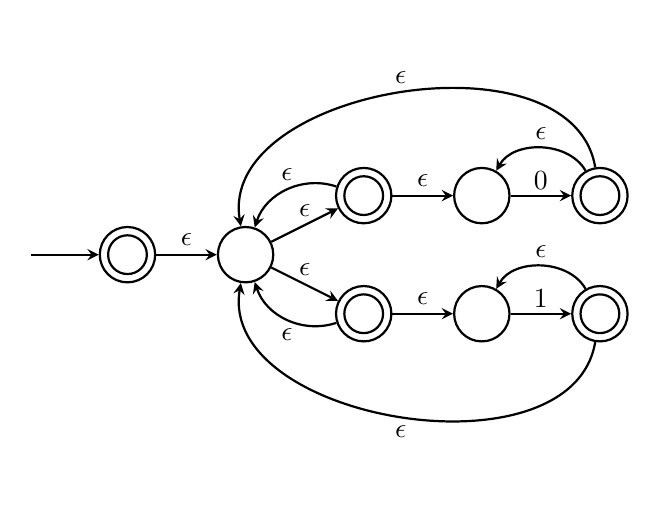
\begin{tikzpicture}
                \begin{scope}[auto, every node/.style={thick, draw,circle,minimum size=2em,inner sep=1}]
                        \node (0) at (0,0) {};
                        \draw[black, thick] (0,0) circle [radius=0.7em];
                        \node (1) at (1.5,0) {};
                        \node (2) at (3,0.75) {};
                        \draw[black, thick] (3,0.75) circle [radius=0.7em];
                        \node (3) at (4.5,0.75) {};
                        \node (4) at (6,0.75) {};
                        \draw[black, thick] (6,0.75) circle [radius=0.7em];
                        \node (5) at (3,-0.75) {};
                        \draw[black, thick] (3,-0.75) circle [radius=0.7em];
                        \node (6) at (4.5,-0.75) {};
                        \node (7) at (6,-0.75) {};
                        \draw[black, thick] (6,-0.75) circle [radius=0.7em];
                \end{scope}
                \node [draw=none, inner sep=0pt] (I) at (-1.25,0) {};
                \begin{scope}[auto, every node/.style={minimum size=1em,inner sep=1}, every path/.style={thick, ->, >=stealth}]
                        \path (I) edge (0);
                        \path (0) edge node {\(\epsilon\)} (1);
                        \path (1) edge node [above] {\(\epsilon\)} (2);
                        \path (1) edge node [above] {\(\epsilon\)} (5);
                        \path (2) edge node {\(\epsilon\)} (3);
                        \path (3) edge node {\(0\)} (4);
                        \path (5) edge node {\(\epsilon\)} (6);
                        \path (6) edge node {\(1\)} (7);
                        \path (4) edge [bend right=60] node [above] {\(\epsilon\)} (3);
                        \path (7) edge [bend right=60] node [above] {\(\epsilon\)} (6);
                        \path (2) edge [bend right=45] node [above] {\(\epsilon\)} (1);
                        \path (4) edge [bend right=90] node [above] {\(\epsilon\)} (1);
                        \path (5) edge [bend left=45] node [below] {\(\epsilon\)} (1);
                        \path (7) edge [bend left=90] node [below] {\(\epsilon\)} (1);
                \end{scope}
        \end{tikzpicture}
\end{center}

\section*{Problem 3}

We can write a regular expression for this language \(L_3\), which shows that it is finite state. Let \(x\) be a string in the set
\[\{aaa, aab, aba, abb, baa, bab, bba, bbb\}\]
and \(R\) be some constant. Then the regular expression
\[E_x = (\Sigma^*x\Sigma^*x^R\Sigma^*) \cup (\Sigma^*x^R\Sigma^*x\Sigma^*)\]
denotes a string in \(L_3\) that contains a given \(x\) and \(x^R\). Then we have that
\[L_3=E_{aaa} \cup E_{aab} \cup E_{aba} \cup E_{abb} \cup E_{baa} \cup E_{bab} \cup E_{bba} \cup E_{bbb}\]
which is a regular expression that proves that \(L_3\) is a finite state language.

\section*{Problem 4}

\paragraph{a)}

\begin{center}
        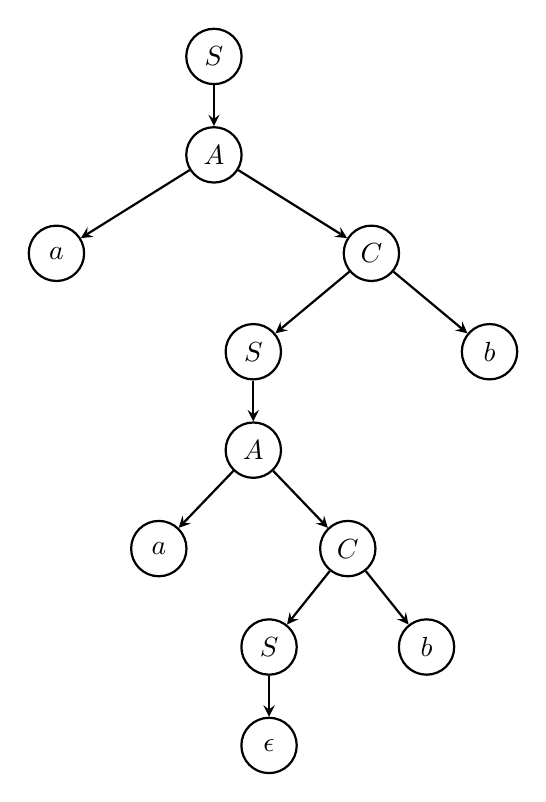
\begin{tikzpicture}
                \begin{scope}[auto, every node/.style={thick, draw,circle,minimum size=2em,inner sep=1}]
                        \node (S1) at (0,0) {\(S\)};
                        \node (A1) at (0,-1.25) {\(A\)};
                        \node (a1) at (-2,-2.5) {\(a\)};
                        \node (C1) at (2,-2.5) {\(C\)};
                        \node (S2) at (0.5,-3.75) {\(S\)};
                        \node (b1) at (3.5,-3.75) {\(b\)};
                        \node (A2) at (0.5,-5) {\(A\)};
                        \node (a2) at (-0.7,-6.25) {\(a\)};
                        \node (C2) at (1.7,-6.25) {\(C\)};
                        \node (S3) at (0.7,-7.5) {\(S\)};
                        \node (b2) at (2.7,-7.5) {\(b\)};
                        \node (Ep) at (0.7,-8.75) {\(\epsilon\)};
                \end{scope}
                \begin{scope}[auto, every node/.style={minimum size=1em,inner sep=1}, every path/.style={thick, ->, >=stealth}]
                        \path (S1) edge (A1);
                        \path (A1) edge (a1);
                        \path (A1) edge (C1);
                        \path (C1) edge (S2);
                        \path (C1) edge (b1);
                        \path (S2) edge (A2);
                        \path (A2) edge (a2);
                        \path (A2) edge (C2);
                        \path (C2) edge (S3);
                        \path (C2) edge (b2);
                        \path (S3) edge (Ep);
                \end{scope}
        \end{tikzpicture}
\end{center}

\paragraph{b)}

The leftmost derivation yields the following sequence.
\[S, A, aC, aSb, aAb, aaCb, aaSbb, aabb\]

\pagebreak

\paragraph{c)}

\begin{center}
        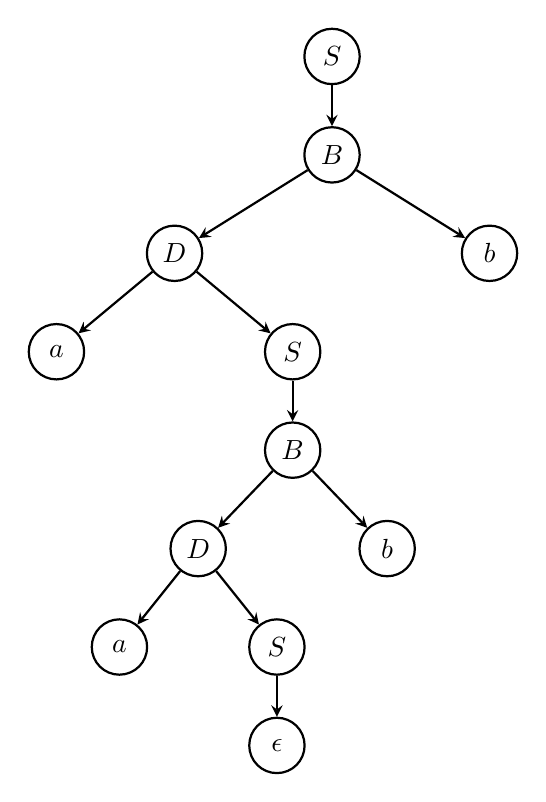
\begin{tikzpicture}
                \begin{scope}[auto, every node/.style={thick, draw,circle,minimum size=2em,inner sep=1}]
                        \node (S1) at (0,0) {\(S\)};
                        \node (B1) at (0,-1.25) {\(B\)};
                        \node (D1) at (-2,-2.5) {\(D\)};
                        \node (b1) at (2,-2.5) {\(b\)};
                        \node (a1) at (-3.5,-3.75) {\(a\)};
                        \node (S2) at (-0.5,-3.75) {\(S\)};
                        \node (B2) at (-0.5,-5) {\(B\)};
                        \node (D2) at (-1.7,-6.25) {\(D\)};
                        \node (b2) at (0.7,-6.25) {\(b\)};
                        \node (a2) at (-2.7,-7.5) {\(a\)};
                        \node (S3) at (-0.7,-7.5) {\(S\)};
                        \node (Ep) at (-0.7,-8.75) {\(\epsilon\)};
                \end{scope}
                \begin{scope}[auto, every node/.style={minimum size=1em,inner sep=1}, every path/.style={thick, ->, >=stealth}]
                        \path (S1) edge (B1);
                        \path (B1) edge (D1);
                        \path (B1) edge (b1);
                        \path (D1) edge (a1);
                        \path (D1) edge (S2);
                        \path (S2) edge (B2);
                        \path (B2) edge (D2);
                        \path (B2) edge (b2);
                        \path (D2) edge (a2);
                        \path (D2) edge (S3);
                        \path (S3) edge (Ep);
                \end{scope}
        \end{tikzpicture}
\end{center}

\paragraph{d)}

The leftmost derivation yields the following sequence.
\[S, B, Db, aSb, aBb, aDbb, aaSbb, aabb\]

\section*{Problem 5}

Given a starting state \(S\) the following context free grammar describes the language.
\begin{align*}
        S &\rightarrow LR\\
        L &\rightarrow aLb\mid\epsilon\\
        R &\rightarrow bRc\mid\epsilon\\
\end{align*}

\end{document}